El esquema del filtro propuesto es el de la figura \ref{fig:filtro_adaptativo}. Ambos sistemas se excitan con una señal de referencia $u(n)$ de ruido blanco gaussiano, produciendo cada uno una salida. Se computa la diferencia entre ambas salidas y se utiliza esta señal de error para el ajuste de los parametros del filtro mediante algun algoritmo adaptativo. Cuando el filtro aprenda a comportarse igual que el sistema a identificar, el error será bajo, y los coeficientes del filtro podrán utilizarse como estimadores de los parametros del sistema a identificar.

\vspace*{\fill}
\begin{figure}[H]
\centering
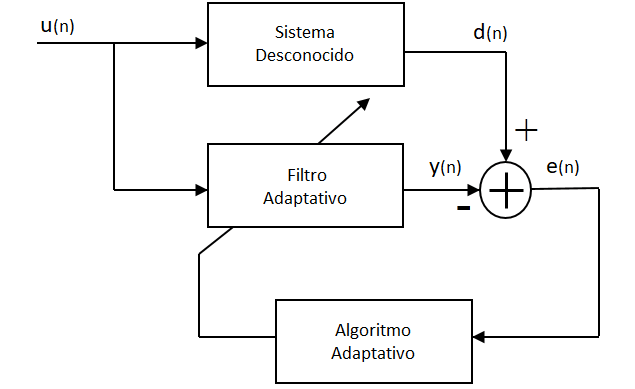
\includegraphics[scale=0.5]{filtro_adaptativo.png}
\caption{Filtro Adatptativo.}
\label{fig:filtro_adaptativo} 
\end{figure}
\vspace*{\fill}

Ahora bien, esto tiene un problema. La salida de nuestro filtro adaptativo se computa de la siguiente manera:

\begin{equation*}
	y(n) = w^T U(n)
\end{equation*}

Donde $U(n) = [u(n) \> u(n - 1) \> ... \> u(n - M + 1)]^T$, $M$ es el orden del filtro y $w$ son los coeficientes del mismo. Esto significa que nuestro filtro adaptativo sólo nos sirve para estimar la respuesta en frecuencia de sistemas FIR y nuestro sistema tiene la forma de un filtro IIR en tiempo discreto:

\begin{equation*}
		x_{0}(n) = b_{0} \> x_{1}(n) + b_{1} \> x_{1}(n - 1) + a_{0} \> x_{0}(n - 1) + a_{1} \> x_{0}(n - 2)
\end{equation*}

Una posible solución a esto es, en lugar de solo meter ruido blanco a la entrada, meter el ruido blanco y algunos valores pasados de la salida:

\begin{equation*}
	U(n) = [x_{1}(n) \> x_{1}(n - 1) \> x_{0}(n - 1) \> x_{0}(n - 2)]^T
\end{equation*}

Donde ahora estamos excitando al sistema con $x_{1}$ ruido blanco gaussiano. Ahora los coeficientes $w$ ajustados del filtro podran utilizarse como estimadores:

\begin{equation*}
	[w_{0} \> w_{1} \> w_{2} \> w_{3}]^T  = [\hat{b}_{0} \> \hat{b}_{1} \> \hat{a}_{0} \> \hat{a}_{1}]^T
\end{equation*}

Ahora bien, como estos coeficientes son función de las constantes $M$, $b$ y $k$, pueden estimarse las mismas. El unico componente que falta es la elección del algoritmo adaptativo. Se propone en principio utilizar el algoritmo LMS, que obtiene los parametros $w$ de la siguiente manera:

\begin{equation*}
	w(n) = w(n - 1) + \mu \> U(n) \> [d(n) - U(n)^* w(n - 1)]
\end{equation*}

Donde $\mu$ es una constante de aprendizaje.
